\documentclass[11pt,letterpaper,titlepage]{article}
\usepackage{fancyhdr}
\usepackage[left=0.75in, right=0.75in, bottom=1.0in]{geometry}
\usepackage{lastpage}
\usepackage{titleref}
\usepackage{booktabs}
\usepackage{appendix}
\appendixtitleon
\appendixtitletocon

\makeatletter

%================== List of figures and tables mods
\usepackage{tocloft}
\usepackage[labelfont=bf]{caption}

\renewcommand{\cftfigpresnum}{Figure\ }
\renewcommand{\cfttabpresnum}{Table\ }

\newlength{\mylenf}
\settowidth{\mylenf}{\cftfigpresnum}
\setlength{\cftfignumwidth}{\dimexpr\mylenf+1.5em}
\setlength{\cfttabnumwidth}{\dimexpr\mylenf+1.5em}



%=================== Graphics
\usepackage{graphicx}
\usepackage[breakwords]{truncate}
\usepackage{float}
\usepackage{array}
\usepackage{amsmath}
\usepackage{mdframed}
\usepackage{fancyvrb}
\usepackage{float}
\usepackage{cancel}
\usepackage{amssymb}
\graphicspath{ {images/} }
\usepackage[usenames,dvipsnames,svgnames,table]{xcolor}
\usepackage[defaultlines=2,all]{nowidow}
\usepackage{listings}
\usepackage{color}
\definecolor{Brown}{cmyk}{0,0.81,1,0.60}
\definecolor{OliveGreen}{cmyk}{0.64,0,0.95,0.40}
\definecolor{CadetBlue}{cmyk}{0.62,0.57,0.23,0}
\usepackage{pdflscape}
\usepackage{relsize}
\usepackage{verbatim}
\usepackage{tabto}


%=================== Settings
\renewcommand{\baselinestretch}{1.2}
\definecolor{gray}{rgb}{0.4 0.4 0.4}
\newcommand{\stimes}{{\times}}

\begin{document}
\newcommand{\NSCDOCNUMBR}{NSC-REP-15-X}         %Put document number here
\newcommand{\NSCDOCSUBJT}{TECHNICAL REPORT: }   %Put document subject here
\newcommand{\NSCDOCTITLE}{$PKINETICS$ - Nuclear Fission Reactor Point Kinetics in $JIC^{Lib2}$}       %Put document title here
\newcommand{\NSCDOCDATE} {March, 2016}    %Put document date here
\newcommand{\NSCDOCREV}  {Rev 1.01} %Put revision number here

\lstset{language=C++,frame=ltrb,framesep=4pt,basicstyle=\linespread{0.8} \small,
	keywordstyle=\ttfamily\color{OliveGreen},
	identifierstyle=\ttfamily\color{CadetBlue}\bfseries,
	commentstyle=\color{Brown},
	stringstyle=\ttfamily,
	showstringspaces=ture }


%################################# TITLE PAGE ########################
\begin{titlepage}
	\pagestyle{fancy}
	\vspace*{1.0cm}
	\centering
	%\includegraphics{NSC_Logo} \par
	\vspace{1cm}
	%\centering
	%{\Large\bfseries  \NSCDOCNUMBR   \par}
	\vspace{.25cm}
	%\centering
	{\Large\bfseries  \NSCDOCSUBJT \par} 
	{\Large\bfseries \NSCDOCTITLE  \par}
	\vspace{1cm}
	{\Large \NSCDOCDATE \par}
	\vspace{1.0cm}
	{\Large Jan Vermaak \& Guillermo Villanueva \par}
	{\Large \NSCDOCREV \par}
		
	\begin{comment}
	\renewcommand{\arraystretch}{2.0}
	\begin{tabular}{| m{2.5cm} | m{4.5cm} | m{4.5cm} |}
		\cline{2-3}
		\multicolumn{1}{c|}{} & \bfseries{Name} & \bfseries{Signature \& Date} \\ \hline
		\bfseries{Prepared} &     &     \\ \hline
		\bfseries{Reviewed} &     &     \\ \hline
		\bfseries{Reviewed} &     &     \\ \hline
	    \bfseries{Approved} &     &     \\ \hline
	\end{tabular} \par
	\end{comment}
	\begin{center}
		\begin{minipage}[c]{0.55\textwidth}
	
			\begin{figure}[H]
			
				
\includegraphics{Logo.png}
			\end{figure}
		\end{minipage}
	\end{center}
	\vspace{2cm}
	%NSC-FRM-15-1 Rev.1
\end{titlepage}


\pagestyle{fancy}
\rfoot{Page \thepage \ of \pageref{LastPage}}
%\cfoot{NSC-FRM-15-1 Rev.1}
\cfoot{}
\lfoot{\truncate{14cm}{\NSCDOCTITLE}}
\rhead{}
\chead{\currentname}
\lhead{}
\renewcommand{\footrulewidth}{0.4pt}
\tableofcontents
\addtocontents{toc}{~\hfill\textbf{Page}\par}

\listoffigures
\listoftables
\chead{Contents}


\newpage
\chead{1 Derivation of the Point Kinetics Equations}
\section{Derivation of the Point Kinetics Equations}

A very simple approximation of the kinetics of a reactor can be made by integrating the neutron transport equation over the entire core volume. This results in the reduced transport equation as shown below:

\begin{equation}
\begin{aligned}
\frac{1}{v}\frac{d\phi}{dt}+\nabla \vec{J} + \Sigma_a \phi(t) &= (1-\beta_{\mathrm{eff}})\bar{\nu} \Sigma_f \phi (t) + \sum_{i=1}^6 \lambda_i C_i (t) \\
\frac{dC_i}{dt} &= \beta_{i,\mathrm{eff}}\bar{\nu} \Sigma_f \phi (t) - \lambda_i C_i (t) \quad i=1,\dots,6 \\
\end{aligned}
\end{equation}

\noindent
Where:\newline
\begin{tabular}{ m{0.75cm}  m{13cm}  }
		$\nu$  &, Neutron velocity [m.s$^{-1}$]        \\ 
		$\phi$ &, Average neutron flux [cm$^{-2}$.s$^{-1}$]   \\ 
		$\vec{J}$ &, Neutron current [cm$^{-2}$.s$^{-1}$] \\
		$\Sigma_a$ &, Effective macroscopic absorption cross-section [cm$^{-1}$] \\
		$\beta_{\mathrm{eff}}$ &, Effective delayed neutron fraction \\
		$\bar{\nu}$ &, Average amount of neutrons released per fission \\
		$\Sigma_f$ &, Effective macroscopic fission cross-section [cm$^{-1}$] \\
		$\lambda_i$ &, Decay constant for delayed neutron precursor i [s$^{-1}$] \\
		$C_i$ &, Average concentration of delayed neutron precursor i [cm$^{-3}$] \\
		$\beta_{i,\mathrm{eff}}$ &, Effective delayed neutron fraction of precursor i \\
\end{tabular} 
\newline
\newline
\newline
\noindent
In order to simplify equation 1 we need to define three additional parameters, the multiplication factor, $k_{\mathrm{eff}}$, the prompt neutron lifetime, $l_p$, and reactivity, $\rho$.

\subsection{The effective multiplication factor, $k_{\mathrm{eff}}$}

To get some context on where we will use this parameter we first lump all the components of criticality together as follows:

\begin{equation}
\begin{aligned}
	\frac{1}{v}\frac{d\phi}{dt} &= (1-\beta_{\mathrm{eff}})\bar{\nu} \Sigma_f \phi (t) -\nabla \vec{J} - \Sigma_a \phi(t)+ \sum_{i=1}^6 \lambda_i C_i (t) \\
	 &= \bar{\nu} \Sigma_f \phi (t)\biggr((1-\beta_{\mathrm{eff}})-\biggr(\frac{\nabla \vec{J} + \Sigma_a \phi(t)}{\bar{\nu} \Sigma_f \phi (t)}\biggr)\biggr) + \sum_{i=1}^6 \lambda_i C_i (t) \\
\end{aligned}
\end{equation}
We then define the effective multiplication factor as the ratio of sources to losses (i.e. $\frac{\mathrm{born}}{\mathrm{lost}}$):

\begin{equation}
	k_{\mathrm{eff}}=\frac{(1-\beta_{\mathrm{eff}})\bar{\nu} \Sigma_f \phi (t) + \sum_{i=1}^6 \lambda_i C_i (t)}{\nabla \vec{J} + \Sigma_a \phi(t)}
\end{equation}

\vspace{0.25cm}\noindent
The next parameter, the prompt neutron lifetime, $l_p$, is a parameter that is both defined and measured at steady state. Therefore, at steady state, all the $\frac{dC_i}{dt}$ terms in equation 1 reduce to zero and we can deduce: 
$$
\lambda_i C_i (t)=\beta_{i,\mathrm{eff}}\bar{\nu} \Sigma_f \phi (t)
$$ 
\noindent
Therefore:

\begin{equation*}
\begin{aligned}
\sum_{i=1}^6 \lambda_i C_i (t) &= \sum_{i=1}^6 \beta_{i,\mathrm{eff}}\bar{\nu} \Sigma_f \phi (t) \\
&=\bar{\nu} \Sigma_f \phi (t) \biggr( \sum_{i=1}^6 \beta_{i,\mathrm{eff}} \biggr) \\
\sum_{i=1}^6 \lambda_i C_i (t) &=\beta_{\mathrm{eff}}\bar{\nu} \Sigma_f \phi (t)
\end{aligned}
\end{equation*}
\noindent
Equation 3 then becomes:
\begin{equation*}
\begin{aligned}
	k_{\mathrm{eff}}&=\frac{(1-\beta_{\mathrm{eff}})\bar{\nu} \Sigma_f \phi (t) + \beta_{\mathrm{eff}}\bar{\nu} \Sigma_f \phi (t)}{\nabla \vec{J} + \Sigma_a \phi(t)} \\
	\therefore k_{\mathrm{eff}} &=\frac{\bar{\nu} \Sigma_f \phi (t) }{\nabla \vec{J} + \Sigma_a \phi(t)} \\
\end{aligned}
\end{equation*}
\noindent
Substituting this value of $k_{\mathrm{eff}}$ into equation 2, one obtains:
\begin{equation}
	\frac{1}{v}\frac{d\phi}{dt}=\bar{\nu} \Sigma_f \phi (t)\biggr((1-\beta_{\mathrm{eff}})-\frac{1}{k_{\mathrm{eff}}}\biggr) + \sum_{i=1}^6 \lambda_i C_i (t) \\
\end{equation}
\noindent
Next we will remove the $\bar{\nu} \Sigma_f$ term by defining the prompt neutron lifetime, $l_p$.

\subsection{The prompt neutron lifetime, $l_p$}
The average time from the birth of a prompt neutron to the time it is absorbed or lost is termed the prompt neutron lifetime. In order to derive a more intuitive definition, let us first define the rate of neutron loss (either through absorption or leaking):

$$
\mathrm{rate \ of \ loss} = \mathrm{leakage \ rate + absorption \ rate}
$$
\noindent
This, however, is familiar:
$$
\mathrm{rate \ of \ loss} = \nabla \vec{J} + \Sigma_a \phi(t)
$$
\noindent
It features in the equation for $k_{\mathrm{eff}}$ above and therefore we can write:

$$
\mathrm{rate \ of \ loss}=\frac{\bar{\nu} \Sigma_f \phi (t) }{\nabla \vec{J} + \Sigma_a \phi(t)}\cdot \biggr(   \frac{1}{\bar{\nu} \Sigma_f \phi (t)}  \biggr) = k_{\mathrm{eff}}\cdot \biggr(   \frac{1}{\bar{\nu} \Sigma_f \phi (t)}  \biggr)
$$
The prompt neutron lifetime is then defined as the time it would take to lose a certain neutron population $n(t)$. And this is defined as the total amount lost ($n(t)$) multiplied by the rate of loss:

\begin{equation*}
\begin{aligned}
l_p &=n(t)\times \mathrm{rate \ of \ loss} \\
    &=n(t)\times k_{\mathrm{eff}}\cdot \biggr(   \frac{1}{\bar{\nu} \Sigma_f \phi (t)}  \biggr)\\
\end{aligned}
\end{equation*}
\noindent
Including the definition of flux, $\phi(t)=n(t).v$, we obtain the final form of the prompt neutron lifetime:

\begin{equation*}
\begin{aligned}
l_p&=n(t)\times k_{\mathrm{eff}}\cdot \biggr(   \frac{1}{\bar{\nu} \Sigma_f n(t)v}  \biggr) \\
   &=k_{\mathrm{eff}}\cdot \biggr(   \frac{1}{v.\bar{\nu} \Sigma_f }  \biggr) \\
\therefore l_p &=\frac{k_{\mathrm{eff}}}{v.\bar{\nu} \Sigma_f} \\
\end{aligned}
\end{equation*}
\noindent
Now extraction from this equation an expression for $\bar{\nu} \Sigma_f$ we get:

$$
\bar{\nu} \Sigma_f=\frac{k_{\mathrm{eff}}}{v.l_p}
$$
\noindent
We can then substitute this into equation 4 to obtain:

\begin{equation}
\begin{aligned}
\frac{1}{v}\frac{d\phi}{dt}&=\frac{k_{\mathrm{eff}}}{v.l_p} \phi (t)\biggr((1-\beta_{\mathrm{eff}})-\frac{1}{k_{\mathrm{eff}}}\biggr) + \sum_{i=1}^6 \lambda_i C_i (t) \\
&=\frac{\phi(t)}{v.l_p}\biggr(k_{\mathrm{eff}}(1-\beta_{\mathrm{eff}})-1\biggr) + \sum_{i=1}^6 \lambda_i C_i (t) \\
\end{aligned}
\end{equation}

\subsection{Reactivity $\rho$}
In practical reactor facilities the value of $k_{\mathrm{eff}}$ is never determined in the classical sense because it involves numbers that are hard to comprehend (i.e. 1.001 is controllable whereas 1.01 is a massive excursion). In order to center the concept of criticality around the value of zero (i.e. positive means power increases and negative means power decreases). For this, the term "reactivity", $\rho$, was defined as:

$$
\rho=\frac{k_{\mathrm{eff}}-1}{k_{\mathrm{eff}}}
$$
\noindent
However, the nature of this number was still unsatisfactory since it depended on the kinetic parameter $\beta_{\mathrm{eff}}$. When normalizing by this factor, reactivity, $\rho'$, with units of dollars (\$) becomes analogous between reactor shapes and sizes and is defined by:

\begin{equation}
\rho'=\frac{1}{\beta_{\mathrm{eff}}}\cdot \frac{k_{\mathrm{eff}}-1}{k_{\mathrm{eff}}}
\end{equation}
\noindent
Solving for $k_{\mathrm{eff}}$ from this equation we get:

\begin{equation*}
\begin{aligned}
\rho' &=\frac{1}{\beta_{\mathrm{eff}}}\cdot (1-1/k_{\mathrm{eff}}) \\
\rho'.\beta_{\mathrm{eff}} &=1-1/k_{\mathrm{eff}} \\
1/k_{\mathrm{eff}}  &=1-\rho'.\beta_{\mathrm{eff}} \\
k_{\mathrm{eff}}  &=\frac{1}{1-\rho'.\beta_{\mathrm{eff}}} \\
\end{aligned}
\end{equation*}
\noindent
Substituting this into equation 5 we get:

\begin{equation*}
\begin{aligned}
\frac{1}{v}\frac{d\phi}{dt}&=\frac{\phi(t)}{v.l_p}\biggr(\frac{1}{1-\rho'.\beta_{\mathrm{eff}}}(1-\beta_{\mathrm{eff}})-1\biggr) + \sum_{i=1}^6 \lambda_i C_i (t) \\
&= \frac{\beta_{\mathrm{eff}}(\rho'-1)}{(1-\rho'\beta_{\mathrm{eff}})}\cdot \frac{\phi(t)}{v.l_p}  + \sum_{i=1}^6 \lambda_i C_i (t) \\
\end{aligned}
\end{equation*}

\subsection{Final simplified form}
As a final modification to equation 1 we need to transform the differential equations for the delayed neutron precursors:

$$
	\frac{dC_i}{dt} = \beta_{i,\mathrm{eff}}\bar{\nu} \Sigma_f \phi (t) - \lambda_i C_i (t) \quad i=1,\dots,6
$$
\noindent
We do this by first substituting the derived expression for $\bar{\nu} \Sigma_f $:

$$
	\frac{dC_i}{dt} = \beta_{i,\mathrm{eff}}\frac{k_{\mathrm{eff}}}{v.l_p} \phi (t) - \lambda_i C_i (t) \quad i=1,\dots,6
$$
\noindent
And then the expression for $k_{\mathrm{eff}}$:

$$
\frac{dC_i}{dt} = \beta_{i,\mathrm{eff}}\frac{\frac{1}{1-\rho'.\beta_{\mathrm{eff}}}}{v.l_p} \phi (t) - \lambda_i C_i (t) \quad i=1,\dots,6
$$
\noindent
To finally get:

$$
	\frac{dC_i}{dt} = \frac{\beta_{i,\mathrm{eff}}}{(1-\rho'.\beta_{\mathrm{eff}})}  \cdot   \frac{\phi (t)}{v.l_p}  - \lambda_i C_i (t) \quad i=1,\dots,6
$$
\noindent
Therefore the final simplified form of the point kinetics equations, after substituting the expression for flux ($\phi(t)=n(t).v$) become:

\begin{equation}
\begin{aligned}
\frac{dn}{dt}&= \frac{\beta_{\mathrm{eff}}(\rho'-1)}{(1-\rho'\beta_{\mathrm{eff}})}\cdot \frac{n(t)}{l_p}  + \sum_{i=1}^6 \lambda_i C_i (t) \\
\frac{dC_i}{dt} &= \frac{\beta_{i,\mathrm{eff}}}{(1-\rho'.\beta_{\mathrm{eff}})}  \cdot   \frac{n (t)}{l_p}  - \lambda_i C_i (t) \quad i=1,\dots,6 \\
\end{aligned}
\end{equation}

\newpage
\chead{2 Discretized forms of the Point Kinetics Equations}
\section{Discretized forms of the Point Kinetics Equations}
For any method of discretization, the time derivatives need to be linearized:

$$
	\frac{dn}{dt}=\frac{n^{j+1}-n^j}{\Delta t}
$$
$$
	\frac{dC_i}{dt}=\frac{C_i^{j+1}-C_i^j}{\Delta t}
$$
\newline
\noindent
Where $j$ and $j+1$ refers to time steps in the solution domain.


\subsection{Initial first-order discretization by uncoupling}
As an initial approach, let us consider calculating the future time step by strictly using values from the previous time step. This is known as Euler's Method for numerically solving ordinary differential equations:

\begin{equation*}
\begin{aligned}
\frac{n^{j+1}-n^j}{\Delta t}&= \frac{\beta_{\mathrm{eff}}(\rho'-1)}{(1-\rho'\beta_{\mathrm{eff}})}\cdot \frac{n^j}{l_p}  + \sum_{i=1}^6 \lambda_i C_i^j \\
\frac{C_i^{j+1}-C_i^j}{\Delta t} &= \frac{\beta_{i,\mathrm{eff}}}{(1-\rho'.\beta_{\mathrm{eff}})}  \cdot   \frac{n^j}{l_p}  - \lambda_i C_i^j \quad i=1,\dots,6 \\
\end{aligned}
\end{equation*}
\newline
\noindent
In this form, each of the 7 equations can be calculated individually (uncoupled form) and the implementation in computer code becomes fairly easy:
\begin{equation}
\begin{aligned}
n^{j+1}&=n^j + \Delta t \biggr(  \frac{\beta_{\mathrm{eff}}(\rho'-1)}{(1-\rho'\beta_{\mathrm{eff}})}\cdot \frac{n^j}{l_p}  + \sum_{i=1}^6 \lambda_i C_i^j \biggr) \\
C_i^{j+1}  &=C_i^j +  \Delta t \biggr(  \frac{\beta_{i,\mathrm{eff}}}{(1-\rho'.\beta_{\mathrm{eff}})}  \cdot   \frac{n^j}{l_p}  - \lambda_i C_i^j \biggr) \quad i=1,\dots,6 \\
\end{aligned}
\end{equation}
\newline
\noindent
The detriment of this method however is that it is fairly unstable and induces large errors when the time step is not extremely small.

\subsection{Problems with the coupled version}
The set of equations 7, is a system of coupled linear ordinary differential equations. By applying the first order discretization, as we did above, where we solve each equation by using the previous time step values we essentially make them uncoupled and hence easy to solve. However, this approach introduces instability and an error between time steps that can only be minimized by using very small time steps. In order to improve the stability and the cumulative error we must use the system of equations in their coupled form:
\begin{equation*}
\begin{aligned}
\frac{n^{j+1}-n^j}{\Delta t}&= \frac{\beta_{\mathrm{eff}}(\rho'-1)}{(1-\rho'\beta_{\mathrm{eff}})}\cdot \frac{n^{j+1}}{l_p}  + \sum_{i=1}^6 \lambda_i C_i^{j+1} \\
\frac{C_i^{j+1}-C_i^j}{\Delta t} &= \frac{\beta_{i,\mathrm{eff}}}{(1-\rho'.\beta_{\mathrm{eff}})}  \cdot   \frac{n^{j+1}}{l_p}  - \lambda_i C_i^{j+1} \quad i=1,\dots,6 \\
\end{aligned}
\end{equation*}
\newline
\noindent
In order to make this equation a little easier to read let us group some values that are constant over the time step:
$$
A_0=\Delta t.\frac{\beta_{\mathrm{eff}}(\rho'-1)}{(1-\rho'\beta_{\mathrm{eff}})}\cdot \frac{1}{l_p}
$$
$$
A_i=\Delta t.\frac{\beta_{i,\mathrm{eff}}}{(1-\rho'.\beta_{\mathrm{eff}})}  \cdot   \frac{1}{l_p} \quad i=1,\dots,6 
$$
And:
$$
\Lambda_i = \Delta t.\lambda_i
$$
$$
\Lambda_i^*=(1+\Lambda_i)= 1+\Delta t.\lambda_i
$$
And therefore we have a slightly more readable version:
\begin{equation*}
\begin{aligned}
n^{j+1}-n^j&= A_0.n^{j+1}  + \sum_{i=1}^6 \Lambda_i C_i^{j+1} \\
C_i^{j+1}-C_i^j &= A_i.n^{j+1} - \Lambda_i C_i^{j+1} \quad i=1,\dots,6 \\
\end{aligned}
\end{equation*}
\newline
\noindent
Rearranging:
\begin{equation*}
\begin{aligned}
n^{j+1}(1-A_0) - \Lambda_1.C_1^{j+1}- \dots - \Lambda_6.C_6^{j+1}&=n^{j} \\
-A_i.n^{j+1} + \Lambda_i^* .C_i^{j+1} &=   C_i^j\quad i=1,\dots,6 \\
\end{aligned}
\end{equation*}
\newline
\noindent
We can write this in matrix form as: 
\begin{equation*}
\begin{bmatrix}
(1-A_0)	&	-\Lambda_1	&	-\Lambda_2	&	-\Lambda_3	&	-\Lambda_4	&	-\Lambda_5	&	-\Lambda_6 \\
-A_1	&	\Lambda_1^* &	0	&	0	&	0	&	0	&	0	 \\
-A_2	&	0	&	\Lambda_2^* &	0	&	0	&	0	&	0	 \\
-A_3	&	0	&	0	&	\Lambda_3^* &	0	&	0	&	0	 \\
-A_4	&	0	&	0	&	0	&	\Lambda_4^* &	0	&	0	 \\
-A_5	&	0	&	0	&	0	&	0	&	\Lambda_5^* &	0	 \\
-A_6	&	0	&	0	&	0	&	0	&	0	&	\Lambda_6^* 	 \\
\end{bmatrix}
\begin{bmatrix}
n^{j+1} \\
C_1^{j+1} \\
C_2^{j+1} \\
C_3^{j+1} \\
C_4^{j+1} \\
C_5^{j+1} \\
C_6^{j+1} \\
\end{bmatrix}
= 
\begin{bmatrix}
n^{j} \\
C_1^{j} \\
C_2^{j} \\
C_3^{j} \\
C_4^{j} \\
C_5^{j} \\
C_6^{j} \\
\end{bmatrix}
\end{equation*}
In simple matrix form this is:
\begin{equation*}
Ax=b
\end{equation*}
This can then easily be solved using a suitable numerical solver.



\newpage
\chead{3 Thermal feedback}
\section{Thermal feedback}
Thermal feedback has been modeled by including the heat capacity equation:
\newline
$$
\int_{t_i}^{t_f} \dot{Q}.dt=m.C_p.\Delta T
$$
\newline
\noindent
Where the total fuel mass, $m$, and its associated heat capacity, $C_p$, is user supplied. The energy integral $\int_{t_i}^{t_f}\dot{Q}.dt$ is calculated after each time step from:
\newline
$$
\biggr[ \int_{t_i}^{t_f}\dot{Q}.dt   \biggr]^{timestep \ i+1}=\biggr[ \int_{t_i}^{t_f}\dot{Q}.dt   \biggr]^{timestep \ i} + \dot{Q}^{i+1}.\Delta t
$$
\newline
\noindent
The reactor power, $\dot{Q}$, is assumed to be associated with the neutron population through a constant, $C_{power}$, and can be altered from its default unity input by the user. In other words, the following equation is applied:
\newline
$$
\dot{Q}(t)=C_{power}\cdot n(t)
$$
\newline
\noindent
Where $C_{power}=1.0$ by default. The temperature of the fuel is then calculated from:
\newline
$$
T^{i+1}=T^i+\frac{\biggr[ \int_{t_i}^{t_f}\dot{Q}.dt   \biggr]^{timestep \ i+1}}{m.C_p}
$$
\newline
\newline
The default fuel mass in the core corresponds to $90$ TRIGA fuel elements ($90\times 2.461 \ kg.element^{-1}=221.49 \ kg$). For the heat capacity, the heat capacity as a function of temperature have been obtained by weighting the individual heat capacities of pure uranium and zirconium hydride. This approach is justified in NUREG-1282 \cite{NUREG1282}. The heat capacity of Uranium has been obtained from \cite{CpUranium} and that for Zirconium-hydride has been obtained from \cite{CpZircHydride} and are combined in Table \ref{table:fuelCp} below.


\begin{table}[H]
\centering
\caption{Heat capacity of Texas A\&M TRIGA reactor fuel.}
\label{table:fuelCp}
\begin{tabular}{|l|l|l|l|}
\hline
\textbf{Temperature} & \textbf{Heat Capacity} & \textbf{Temperature} & \textbf{Heat Capacity} \\ \hline
\textbf{[K]}           & \textbf{[J/kg/K]}        & \textbf{[K]}           & \textbf{[J/kg/K]}        \\ \hline
323.15               & 216.8                  & 773.15               & 452.3                  \\ \hline
373.15               & 268.8                  & 873.15               & 1577.0                 \\ \hline
473.15               & 321.1                  & 973.15               & 535.6                  \\ \hline
573.15               & 346.3                  & 1073.15              & 430.1                  \\ \hline
673.15               & 399.4                  & 1173.15              & 414.5                  \\ \hline
\end{tabular}
\end{table}
\noindent
The temperature feedback coefficients have been determined from the end-of-life (EOL) data of the Texas A\&M TRIGA Reactor's Safety Analysis Report and the effective temperature feedback is given in Table~\ref{table:reac}.

\begin{table}[H]
\centering
\caption{Reactivity feedback from fuel temperature.}
\label{table:reac}
\begin{tabular}{|l|l|ll}
\hline
\textbf{Temperature {[}K{]}} & \textbf{Reactivity, $\rho$ [\$]} & \multicolumn{1}{l|}{\textbf{Temperature {[}K{]}}} & \multicolumn{1}{l|}{\textbf{Reactivity, $\rho$ [\$]}} \\ \hline
293.15             & 0.000        & \multicolumn{1}{l|}{823.15}             & \multicolumn{1}{l|}{-5.917}       \\ \hline
323.15             & -0.143       & \multicolumn{1}{l|}{873.15}             & \multicolumn{1}{l|}{-6.692}       \\ \hline
373.15             & -0.442       & \multicolumn{1}{l|}{923.15}             & \multicolumn{1}{l|}{-7.505}       \\ \hline
423.15             & -0.819       & \multicolumn{1}{l|}{973.15}             & \multicolumn{1}{l|}{-8.354}       \\ \hline
473.15             & -1.273       & \multicolumn{1}{l|}{1023.15}            & \multicolumn{1}{l|}{-9.208}       \\ \hline
523.15             & -1.865       & \multicolumn{1}{l|}{1073.15}            & \multicolumn{1}{l|}{-10.095}      \\ \hline
573.15             & -2.505       & \multicolumn{1}{l|}{1123.15}            & \multicolumn{1}{l|}{-11.015}      \\ \hline
623.15             & -3.133       & \multicolumn{1}{l|}{1173.15}            & \multicolumn{1}{l|}{-11.968}      \\ \hline
673.15             & -3.816       & \multicolumn{1}{l|}{1223.15}            & \multicolumn{1}{l|}{-12.954}      \\ \hline
723.15             & -4.479       & \multicolumn{1}{l|}{1273.15}            & \multicolumn{1}{l|}{-13.972}      \\ \hline
773.15             & -5.179       &                                         &                                   \\ \cline{1-2}
\end{tabular}
\end{table}
\newpage
\chead{4 Input Guide}
\section{Input Guide}
The \textbf{\textit{pkinetics}} code by default runs a critical system based on the kinetic parameters of the Texas A\&M Nuclear Science Center TRIGA reactor at a neutron population of $0.03 \ neutrons.cm^{-3}$. In order to run the code with different input conditions, an input file can be specified that will alter the conditions of the simulation. As an initial example, consider the input file shown below:


\subsection{Running the code}
The point kinetics code is run by executing \textbf{\textit{JIC\_LIB2.exe }} with the option \textbf{\textit{pkinetics}}, followed by the input file name as shown below: 
\begin{verbatim}
JIC_LIB2.exe pkinetics input.txt
\end{verbatim}

\subsection{Input Cards}
The default values for all the input cards are for the Texas A\&M Nuclear Science Center TRIGA reactor.\newline
\newline
\textbf{beff} {\color{blue} int float} \newline
Specifies the delayed neutron fraction for the delayed neutron precursor group.
\begin{itemize}
	\item Word 1: {\color{blue} int} Delayed neutron precursor group number.
	\item Word 2: {\color{blue} float} Delayed neutron fraction for precursor group.
\end{itemize}
Default values:
\begin{verbatim}
Group 1  2.6457461646E-04 
Group 2  1.4937238494E-03 
Group 3  1.3179916318E-03 
Group 4  2.8312412831E-03 
Group 5  9.0404463040E-04 
Group 6  1.8842398884E-04
\end{verbatim}
\vspace {0.5 cm}

\newpage
\noindent
\textbf{lambda} {\color{blue} int float} \newline
Specifies the decay constant for the delayed neutron precursor group.
\begin{itemize}
	\item Word 1: {\color{blue} int} Delayed neutron precursor group number.
	\item Word 2: {\color{blue} float} Decay constant for precursor group [$s^{-1}$].
\end{itemize}
Default values:
\begin{verbatim}
Group 1  0.01273 
Group 2  0.03171 
Group 3  0.11670 
Group 4  0.31215 
Group 5  1.39880 
Group 6  3.85100 
\end{verbatim}
\vspace {0.5 cm}


\noindent
\textbf{lifetime} {\color{blue} float} \newline
Specifies the prompt neutron lifetime for the simulation.
\begin{itemize}
	\item Word 1: {\color{blue} float} Prompt neutron lifetime [$s$].
\end{itemize}
Default values:
\begin{verbatim}
0.026178e-3
\end{verbatim}
\vspace {0.5 cm}


\noindent
\textbf{precursor} {\color{blue} int float} \newline
Specifies the delayed neutron precursor concentration for the indicated group. If omitted, or values are $0.0$, the zero reactivity steady state values associated with the given population will be used as initial values.
\begin{itemize}
	\item Word 1: {\color{blue} int} Delayed neutron precursor group number.
	\item Word 2: {\color{blue} float} Concentration for precursor group [$cm^{-3}$].
\end{itemize}
Default values:
\begin{verbatim}
Calculate from steady state
\end{verbatim}
\vspace {0.5 cm}


\noindent
\textbf{population} {\color{blue} float} \newline
Specifies the initial neutron population for the simulation.
\begin{itemize}
	\item Word 1: {\color{blue} float} Neutron population [$cm^{-3}$].
\end{itemize}
Default values:
\begin{verbatim}
30.0e-3
\end{verbatim}
\vspace {0.5 cm}

\newpage
\noindent
\textbf{rhopoint} {\color{blue} float float} \newline
Specifies the reactivity versus time dependence. Each time this card appears, the data point goes into an accumulator that will eventually build a time table.
\begin{itemize}
	\item Word 1: {\color{blue} float} Time [$s$].
	\item Word 2: {\color{blue} float} Reactivity [$\$$].
\end{itemize}
Default values:
\begin{verbatim}
0.0  0.0
\end{verbatim}
\vspace {0.5 cm}


\noindent
\textbf{timestep} {\color{blue} float} \newline
Specifies the outer timestep size.
\begin{itemize}
	\item Word 1: {\color{blue} float} timestep [$ms$].
\end{itemize}
Default values:
\begin{verbatim}
0.0166666666
\end{verbatim}
\vspace {0.5 cm}

\noindent
\textbf{simtime} {\color{blue} float} \newline
Specifies the total simulation time.
\begin{itemize}
	\item Word 1: {\color{blue} float} simulation time [$s$].
\end{itemize}
Default values:
\begin{verbatim}
10.0
\end{verbatim}
\vspace {0.5 cm}


\noindent
\textbf{solver} {\color{blue} int} \newline
Specifies the solver selection.
\begin{itemize}
	\item Word 1: {\color{blue} int} Solver option. Can be  {\color{blue}1}:Coupled CG, {\color{blue}2}:Uncoupled Euler.
\end{itemize}
Default values:
\begin{verbatim}
1
\end{verbatim}
\vspace {0.5 cm}

\newpage
\noindent
\textbf{mass} {\color{blue} float} \newline
Specifies the total fuel mass.
\begin{itemize}
	\item Word 1: {\color{blue} float} Fuel mass [$kg$].
\end{itemize}
Default values:
\begin{verbatim}
221.49
\end{verbatim}
\vspace {0.5 cm}


\noindent
\textbf{cpower} {\color{blue} float} \newline
Specifies the power relation to neutron population.
\begin{itemize}
	\item Word 1: {\color{blue} float} ratio.
\end{itemize}
Default values:
\begin{verbatim}
1.0
\end{verbatim}
\vspace {0.5 cm}


\noindent
\textbf{temperature} {\color{blue} float} \newline
Specifies the initial fuel temperature.
\begin{itemize}
	\item Word 1: {\color{blue} float} Fuel temperature [$K$].
\end{itemize}
Default values:
\begin{verbatim}
293.15 K
\end{verbatim}
\vspace {0.5 cm}


\noindent
\textbf{cppoint} {\color{blue} float float} \newline
Specifies the heat capacity dependence on temperature. If so much as a single point is entered, the entire default table is deleted and the new data is accepted.
\begin{itemize}
	\item Word 1: {\color{blue} float} Temperature [$K$].
	\item Word 2: {\color{blue} float} Heat Capacity [$J.kg^{-1}.K^{-1}$].
\end{itemize}
Default values:
\begin{verbatim}
T       Cp      T       Cp
323.15	216.8	773.15	452.3
373.15	268.8	873.15	1577.0
473.15	321.1	973.15	535.6
573.15	346.3	1073.15	430.1
673.15	399.4	1173.15	414.5
\end{verbatim}
\vspace {0.5 cm}

\newpage
\noindent
\textbf{alphapoint} {\color{blue} float float} \newline
Specifies the temperature feedback of the reactor. If so much as a single point is entered, the entire default table is deleted and the new data is accepted.
\begin{itemize}
	\item Word 1: {\color{blue} float} Temperature [$K$].
	\item Word 2: {\color{blue} float} Reactivity [$\$$].
\end{itemize}
Default values:
\begin{verbatim}
T [K]	rho         T [K]	rho
293.15	0.000       823.15	-5.917
323.15	-0.212      873.15	-6.692
373.15	-0.566      923.15	-7.505
423.15	-0.919      973.15	-8.354
473.15	-1.273      1023.15	-9.208
523.15	-1.865      1073.15	-10.095
573.15	-2.505      1123.15	-11.015
623.15	-3.133      1173.15	-11.968
673.15	-3.816      1223.15	-12.954
723.15	-4.479      1273.15	-13.972
773.15	-5.179
\end{verbatim}
\vspace {0.5 cm}

\newpage
\chead{5 Verification \& Validation}
\section{Verification \& Validation}
\subsection{Test 1 - no thermal feedback}
The response of the solver has been measured against the Texas A\&M TRIGA reactor at a power of $300 \ W$. The results are shown in Figure \ref{figure:Test1}. The code matches the reactor data well during withdrawal and insertion of the rod, however, the transition period where withdrawal is reversed the code cannot capture the reactor related transient. Therefore, the code matches well before and after the point where the rod withdrawal direction is changed.

\begin{center}
	\begin{minipage}[c]{0.82\textwidth}

		\begin{figure}[H]
		
			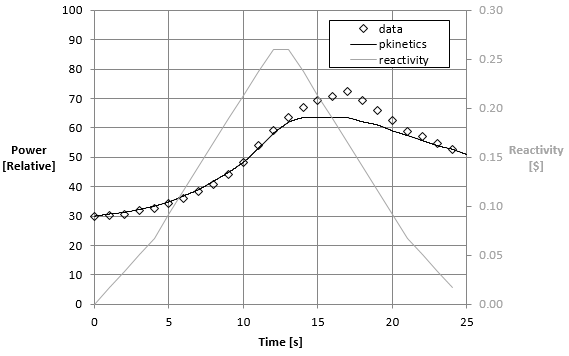
\includegraphics{Test1.png}
			\caption{Results of a simple rod oscillation.}
			\label{figure:Test1}
		\end{figure}
	\end{minipage}
\end{center}

\subsection{Test 2 - Pulsing}
Assessing the performance of the code against measured data is a more strenuous task. The major input parameter(s) is the temperature feedback coefficient. For coefficients obtained from the Texas A\&M TRIGA safety analysis report, for End-of-Life conditions, Table \ref{table:peakPowers} below compares the measured versus calculated values. The values compare within the expected nominal magnitudes, however, given the uncertainty in feedback coefficients this comparison is harder to judge absolute accuracy.

\begin{table}[H]
\centering
\caption{Comparison of peak powers.}
\label{table:peakPowers}
\begin{tabular}{|c|c|c|c|}
\hline
\textbf{Reactivity} & \textbf{Peak NSCR} & \textbf{Peak Code} & \textbf{Deviation} \\
\textbf{{[}\${]}}   & \textbf{{[}MW{]}}  & \textbf{{[}MW{]}}  & \textbf{{[}\%{]}}  \\ \hline
1.15                & 33.2               & 36.1               & 8.9                \\ \hline
1.24                & 64.2               & 81.2               & 26.6               \\ \hline
1.33                & 129.9              & 145.5              & 12.0               \\ \hline
1.56                & 423.8              & 400.6              & -5.5               \\ \hline
\end{tabular}
\end{table}

\begin{center}
	\begin{minipage}[c]{0.82\textwidth}

		\begin{figure}[H]
		
			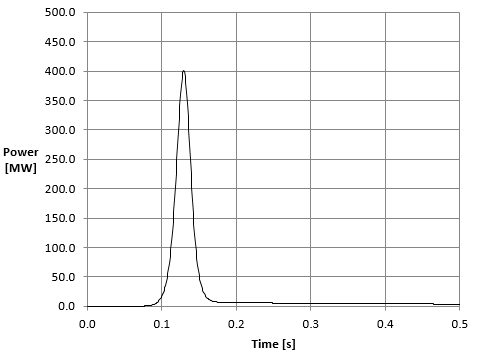
\includegraphics{Test2_Plot.png}
			\caption{Results of a pulse with a reactivity of $\$1.56$.}
			\label{figure:Test2_Plot}
		\end{figure}
	\end{minipage}
\end{center}


\newpage
\chead{6 Example input file}
\section{Example input file}
\begin{verbatim}
// ========================== Kinetic parameters
beff 1  2.6457461646E-04 
beff 2  1.4937238494E-03 
beff 3  1.3179916318E-03 
beff 4  2.8312412831E-03 
beff 5  9.0404463040E-04 
beff 6  1.8842398884E-04 

lambda 1  0.01273 
lambda 2  0.03171 
lambda 3  0.11670 
lambda 4  0.31215 
lambda 5  1.39880 
lambda 6  3.85100 

lifetime 0.026178e-3

// ========================== Simulation initial conditions

precursor 1  0.000
precursor 2  0.000
precursor 3  0.000
precursor 4  0.000
precursor 5  0.000
precursor 6  0.000
population 30.0e-3

// ========================== Reactivity table
rhopoint  0.0    0.0
rhopoint  1.0    0.0
rhopoint  1.0001 0.21

// ========================== Simulation settings
timestep 0.0166666
simtime 10.0
solver 1
\end{verbatim}


\newpage
\chead{References}
\begin{thebibliography}{1}

	\bibitem{NUREG1282} {\em Safety Evaluation Report on High-Uranium Content, Low-Enriched Uranium-Zirconium Hydride Fuels for TRIGA Reactors}, NUREG-1282, Docket number 50-163, GA Technologies, August 1987.
	
	\bibitem{CpUranium} Ginnings D.C., Corruccini R.J., {\em Heat Capacities at High Temperatures of Uranium, Uranium Trichloride, and Uranium Tetrachloride}, Journal of Research of the National Bureau of Standards, Research Paper RP1831, Volume 39, October 1947.
	
	\bibitem{CpZircHydride} Douglas T.B., Victor A.C., {\em Heat Content of Zirconium and of Five Compositions of Zirconium Hydride from $0^{\circ}$ to $990^{\circ}C$}, Journal of Research of the National Bureau of Standards, Research Paper RP2878, Volume 61, July 1958.
	
\end{thebibliography}





\end{document}